\chapter{Overview}
\thispagestyle{empty}
\numberwithin{equation}{chapter}

\section{Problem statement}


\subsection{Dictionaries for signal representation}

%We define an atom is am small unit of something big.
%We define a dictionary is a collection of ordered atoms.

Simplification of signals in signal processing.

As a matter of fact a good dictionary is essential for such a good signal approximation. \cite{} 
Finding good dictionaries has become a major task in the last decades.
There are essential two major distinct ways to construct the desired dictionaries. First the construction of them based on mathematica model and second
via a training process/algorithm from a set of training data.



%copy
% When a signal is said to be sparse in an engineering sense, it really means that the signal can be expanded in either
%a small number of terms or in a series with significantly decaying coefficients. In the former case, one talks about 
%a strictly sparse signal, in the latter case, one talks about a compressible signal. 
%In order to produce Compressed Measurements, one first need to know what is the family of functions in which 
%the signal of interest is sparse. Depending on the case, one might be lucky and know that the signal is sparse in 
%a basis found in harmonic analysis (2.1) or one may have to spend some work in devising what these sparse basis is through 
%an algorithm dedicated to finding sparse dictionaries from a set of signal examples(2.2 and 2.3). 

\subsection{History}

%Compressed sensing
The process of signal transformation that far back in the early 60s.\cite{sparse intro}
FFT in 65s

approximate signals via combination of limited signal samples
Why?
signal analysis, compression, de-noise etc.

The early approaches in the 60s used combinations of cosine transformations. Coming from a continues representation this makes 
actually sense. The signal could be represented via ....

In 80s the search for better transformation basis became a major role in signal representation. \cite{}

%\subsection{Discrete signals}
Rather then using continuous signals we concentrate on discrete signal representation.
Continuous signals would be better for .... . But our signal (image etc.) will be discrete anyway because of their initial digital representation. 
Besides the problem of coding becomes different in the continues space \cite{} Because of ...

\subsection{Splitting the problem}
\cite{Rubinstein2010}
In the last 15 years the concept emerged to interpret basis transforms as a set of signal atoms in a dictionary and the signals 
that they reconstruct as sparse linear combination of these atoms.
see \cite{Olshausen1997} and \cite{}
The benefit of this approach is that you can decouple signal coding and dictionary design.
and split the whole process of signal analysis into two tasks. Coding the signal and design of the dictionary.
Separating the problem into two distinct problems made the search for efficient coding of signals and construction of task specific dictionaries more flexible \cite{?}.

\subsection{Criteria}

Size of database/dictionary
Quality

%In order to find 
%1. coding signals 
%2. find a good dictionary

%analog problem video compression but with less correlation between images and still image 

%Convergence of the dictionary learning
%Quality increase with size increase 
%Comparison with jpeg,jpeg2000 via RMSE


\section{Sparse coding}

The Cambridge Advanced Learner defines a code as ``..a system of numbers, letters or signals which is used to represent something in a shorter or more convenient form''
A sparse code is a sparse vector of coefficients that is used to linear combine a small selection of atoms from a dictionary.

%copy
%In sparse modeling representation, a signal x ∈ Rn is represented as a linear combination of basis column vectors dj ∈ Rn (atoms) which form a dictionary D ∈ Rn×K, such that x = Dα.

Consider $X \in \mathbb{R}^{m\times n}$  as a matrix with $n$ columns each column $x_{i}$ representing a signal described by a single vector of signal length $m$.
The dictionary $D\in\mathbb{R}^{m \times p}$ is another matrix with $p$ columns where each column represents an atom signal with the same dimension and size as a single signal $x_{i}$ from $X$.
The vector $\alpha$ is linear combination of a few non orthonormal atoms from $D$ that is close to the signal $X$.

We try to keep coefficient vector $\alpha$ sparse. 
%Sparse coding is the 
\[
\underbrace{\begin{pmatrix} x_1 \\ x_2 \\ \vdots \\ x_n \end{pmatrix}}_{signal} \approx \underbrace{\begin{pmatrix} d_1  d_2 \cdots d_n \end{pmatrix}}_{\textrm{dictionary atoms}}
\underbrace{\begin{pmatrix} \alpha_1 \\ \alpha_2 \\ \vdots \\ \alpha_n \end{pmatrix}}_{\textrm{keep sparse}}
\]
The solution to this problem is a least-squares solve under-determined linear system we want the sparsest solution.

To achieve the spare solution we add a constraint to the problem. 

\begin{align}
\min_{\alpha\in\mathbb{R}^{p}} \lVert x - D\alpha \rVert^{2}_{2} + \underbrace{\psi(\alpha)}_{regularization}
\end{align}


measure sparsity via       l0-norm       $\lVert\alpha\rVert_{0}$

\begin{figure}
\centering
%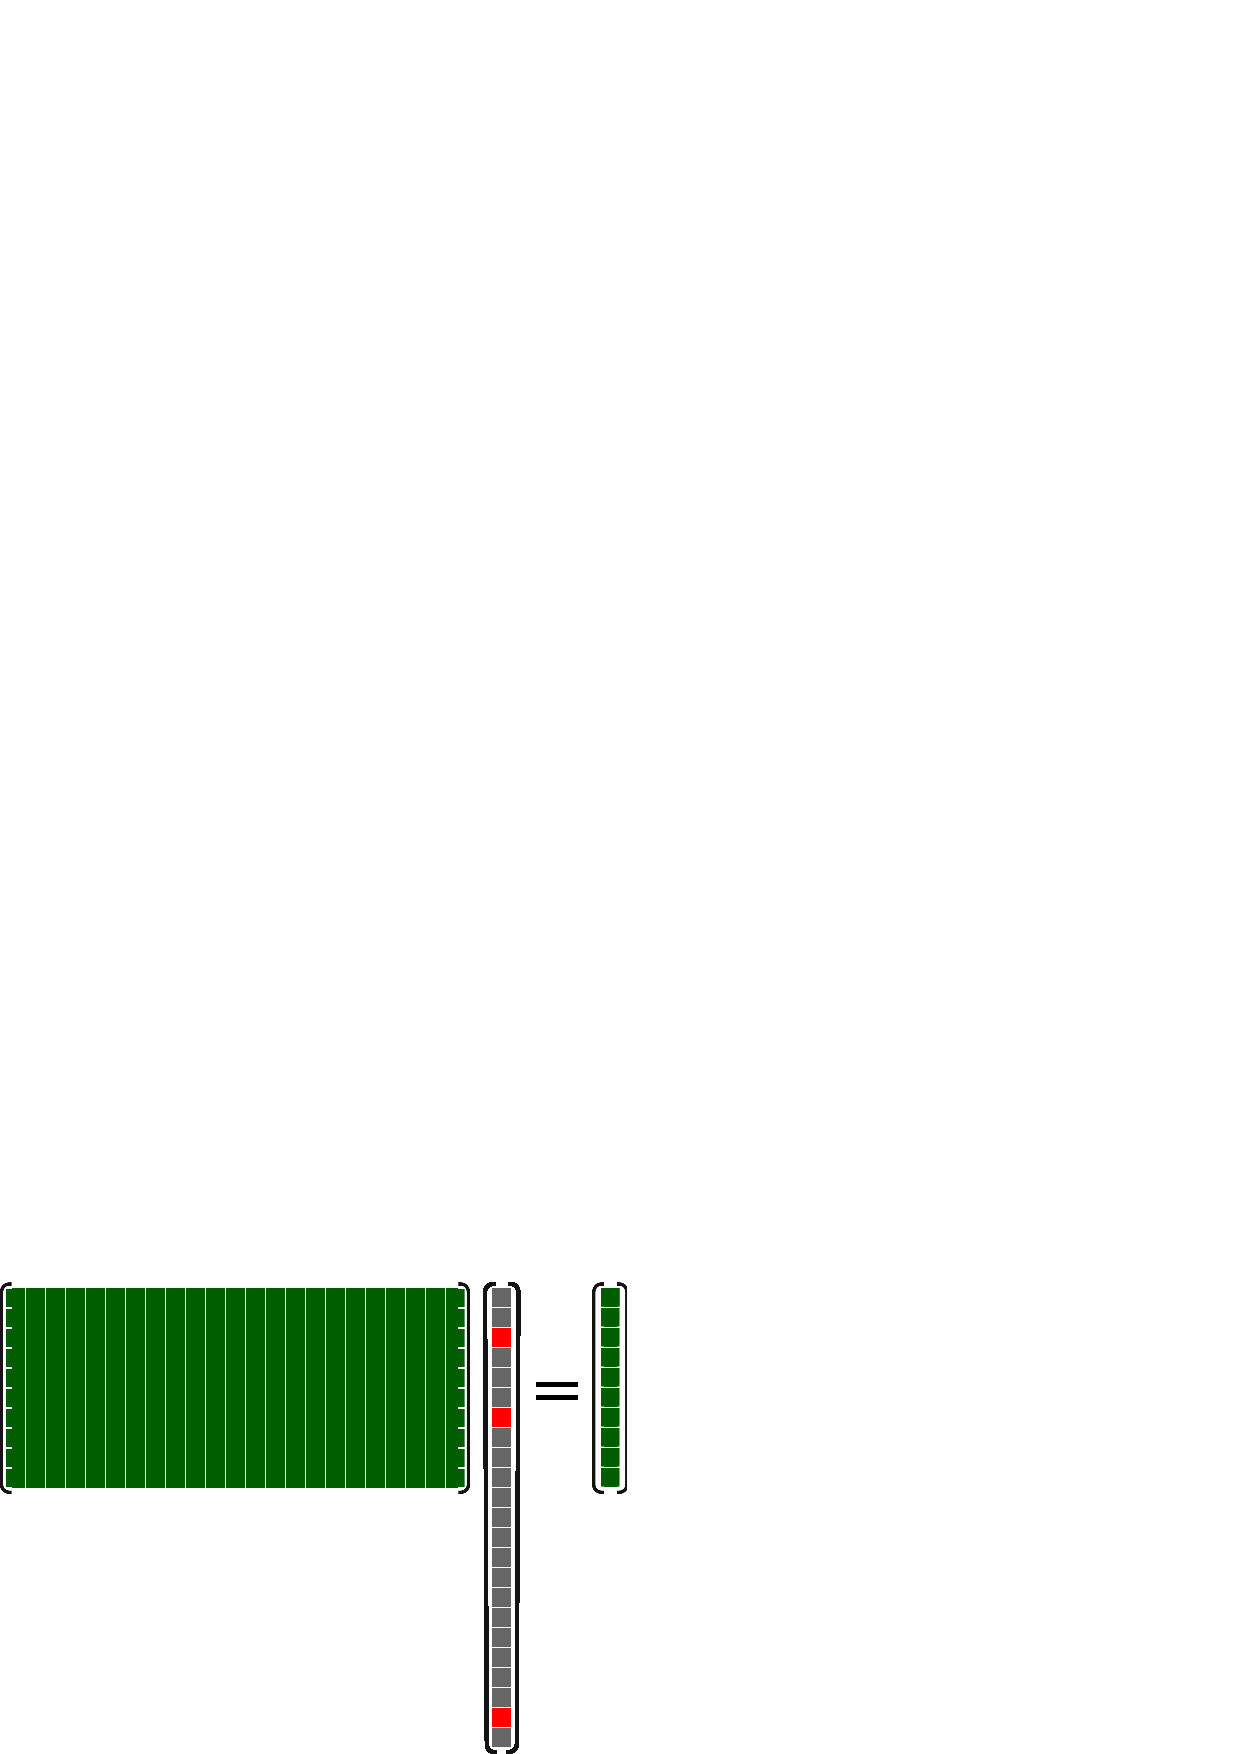
\includegraphics[width = 0.66\textwidth]{images/Da_x.pdf} % Or .pdf
\caption{Sparse Coding}
\label{fig:da_x}
\end{figure}


In the last 15 years several sparse coding algorithms have been proposed. 
Some that solve the initial problem <> greedily, the (orthogonal) matching pursuit, and others which modified the problem to become convex/linear. These primary derive from the numerical domain in the form of 
large linear system solvers with few optimization constraints. The LARS-Lasso, basis pursuit, FOCUSS?

%copy
% Following Tao et al., where it was shown that the L1 norm is equivalent to the L0 norm, 
%leads one to solve an easier problem. Finding the candidate with the smallest L1 norm can be expressed relatively
%easily as a linear program, for which efficient solution methods already exist. These solution methods have been refined over the past few years yielding enormous gain

$\lVert\alpha\rVert_{0}$ makes the problem NP-hard
to get best solution you need to test every combination
Solution:
use greedy approach 

or make problem convex (e.g. use $\lVert\alpha\rVert_{1}$)
the most common algorithms are the following ones.
BP/MP/OMP ...
Lasso/Ridge regression etc.

\Todo{image/description of different regularizations}


\subsection {$\ell_0$ regularization with greedy algorithm}

The algorithm calculates a coefficient vector $\alpha$ which is an greedy/approximate solution of the following NP-hard problem
\begin{align}
\min_{\alpha\in\mathbb{R}^{p}}  \lVert x - D\alpha \rVert^{2}_{2} \textrm{ s.t. } \lVert \alpha \rVert_{0} \leq L
\end{align}
or
\begin{align}
\min_{\alpha\in\mathbb{R}^{p}}   \lVert \alpha \rVert_{0}   \textrm{ s.t. } \lVert x - D\alpha \rVert^{2}_{2} \leq \epsilon
\end{align}
\cite{Mallat1993}

\subsection*{Matching pursuit}
\begin{algorithm}
\begin{algorithmic}
\STATE i=0
\end{algorithmic}
\end{algorithm}

\subsubsection{Orthogonal matching pursuit}
\cite{Pati1993}
\label{sec:omp}

%copy
%OMP to address the NP-hard sparse coding problem

\begin{algorithm}
\caption{Orthogonal-Matching-Pursuit}
\begin{algorithmic}[1]
\REQUIRE $x \in \mathbb{R}^m, y \in \mathbb{R}^m, D \in \mathbb{R}^{m\times k}, \epsilon \in \mathbb{R}$
\STATE $\alpha_o \gets 0, r_0 \gets x $ (residual) $, S_0=\emptyset$
\FOR {$i = 1$ to $L$}
\STATE Select atom with maximum correlation with residual: 
\begin{equation*}
i \gets \argmax_{i=1,...,p} \lvert d_i^Tr \rvert
\end{equation*}
\STATE update active set: $S \gets S \cup \{i\} $
\STATE update residual: $r \gets \left(I-D_S\left( D_S^T D_S \right)^{-1} D_S^T \right)x$
\STATE update coefficients: $a_S \gets \left( D_S^T D_S \right)^{-1} D_S^T x $

\ENDFOR
\RETURN $\alpha$
\end{algorithmic}
\end{algorithm}

\subsection {$\ell_1$ regularization}

basis pursuit\cite{} 
FOCUSS \cite{}

The LASSO (least absolute shrinkage and selection operator) is a regularized version of a least squares solution.
The regularized version is found by adding a constraint that induces the $L_1$-norm of the solution to be small. \cite{Tibshirani1998}
There are several ways to compute the LASSO. .. ...... \cite{} 

\subsubsection {LARS-Lasso}
\label{sec:lars}
The LARS-Lasso is a algorithm to solve the LASSO with the help of least angle regression (short LAR)
as described in \cite{Efron2004}. It is a modified version of the LAR where .... variables are removed when they cross zero ...


\begin{align}
\min_{\alpha\in\mathbb{R}^{p}}  \frac{1}{2} \lVert x - D\alpha \rVert^{2}_{2} + \lambda \lVert \alpha \rVert_{1}
\end{align}

\Todo{add algo.}
\begin{algorithm}
\caption{LARS-lasso}
\begin{algorithmic}[1]
\REQUIRE $x \in \mathbb{R}^m$
\end{algorithmic}
\end{algorithm}

\subsubsection*{Limitations}
The Lasso modified version of the LAR hat the following limitations.
\begin{description}
 \item[Dimension] to high dimension of signal When the dimension $p$ of the signal $X$ is 
much higher than the the dimension $m$ of the dictionary $D$ the algorithm can only select $m$ columns.

\item[correlation] When the columns of the dictionary are highly correlated the algorithm
selects only one column.
\end{description}

Limitation one is irrelevant for our experiments as the dictionaries are over-complete 
, with respect to the dimension $m$ of signal $X$, and thus satisfy $p\leq n$.





\section{Dictionaries}
\subsection{Structure}
\subsubsection*{Designed}
\begin{description}
 \item[cosine]
 \item[wavelets]
 \item[curvelets/contourlets/bandelets]
\end{description}

\subsubsection*{Learned}
Recent research has shown that learned dictionaries show better compression quality than small analytic dictionaries \cite{Aharon2006} \cite{Chen1998} 
Rather than selecting an appropriate mathematical construct that can reconstruct a certain group of signals close enough the data, a subset or similar data
is used as a training set to generate the dictionary itself.


%\subsubsection{k-svd}
\subsection{Learning}
In the last decade several learning algorithms have been proposed.
The basic concept of following algorithms for learning redundant dictionaries is to alter a initial start dictionary
in this way that it can sparsely reconstruct a set of training data with minimal error. 

\subsubsection*{Batch}
MOD \cite{Engan1999}
Generalized PCA \cite{}
ILS-DLA \cite{}
K-SVD \cite{Aharon2006}


\subsubsection*{Online}
In 2010 new training algorithms were presented that enabled on-line learning of dictionaries. 
In contrast to batch learning algorithms with a fixed training set the new approaches enabled
This is good for very large training sets or training data that is unknown at the start of the training process.

... RLS-DLA \cite{Engan2010} ...

\Todo{find the Japanese one}

In 2010 Mairal et. al. \cite{Mairal2010} proposed an on-line approach which from now on will be called TrainDL

\subsubsection*{TrainDL}
\label{sec:mairal}
The algorithm presented by Mairal et al. \cite{Mairal2010} is ...

\begin{algorithm}
\caption{Online dictionary learning \cite{Mairal2010}}
\begin{algorithmic}[1]
\REQUIRE $x \in \mathbb{R}^m,  p \left( x \right), \lambda \in \mathbb{R}, D_0 \in \mathbb{R}^{m \times p}, T$
\STATE $A_0 \in \mathbb{R}^{p \times p} \gets  0, B_0 \in \mathbb{R}^{m \times p}\gets 0$
\FOR {$t = 1$ to $T$}
\STATE Draw $x$ from p(x).
\STATE Sparse code:
\begin{align} 
\alpha_t \equiv \argmin_{\alpha\in\mathbb{R}^{p}}  \lVert x_t - D_t\alpha \rVert^{2}_{2}  +  \lambda \lVert \alpha \rVert_{1}
\end{align}

\STATE $A_t \gets A_{t-1} + \alpha_t\alpha_t^T$
\STATE $B_t \gets B_{t-1} + x_t\alpha_t^T$
\STATE Compute $D_t$ using \prettyref{alg:update}, with $D_{t-1}$ as warm restart 
\begin{align} 
D_t \equiv \argmin_{D \in \mathbb{R}^{m x k}}  \frac{1}{t} \sum_{i=1}^t \left( \lVert x_i - D\alpha_i \rVert^{2}_{2}  +  \lambda \lVert \alpha_i \rVert_{1} \right) \label{eq:update}
\end{align}
\ENDFOR
\RETURN $D_T$
\end{algorithmic}
\end{algorithm}


\begin{algorithm}
\caption{Dictionary Update}
\label{alg:update}
\begin{algorithmic}[1]
\REQUIRE $D=[d_1,...,d_p] \in \mathbb{R}^{m \times p}, A=[a_1,...,a_p] \in \mathbb{R}^{p \times p}, B=[b_1,...,b_p] \in \mathbb{R}^{m \times p}$
\REPEAT
\FOR {$j = 1$ to $p$}
\STATE update j-th column to optimze for \prettyref{eq:update}:
\begin{align}
u_j \gets \frac{1}{A[j,j]}\left(b_j-Da_j\right)+d_j \\
d_j \gets \frac{1}{\max\left(\lVert u_j \rVert_2,1\right)} u_j
\end{align}

\ENDFOR
\UNTIL convergence 
\RETURN $D$
\end{algorithmic}
\end{algorithm}

\subsection{Application}

\begin{description}
\item[noise reduction]
Remove noise from a signal. Using the fact that sparse coding 
is an approximation of signal that looses .... in its encoding process. 
\cite{Elad2006}

\item[in-painting]
fill missing parts by removing rows from the dictionary
Train with the original image
\cite{mairal08sparse}

\item[compression] An example for this is the compression of facial images by Bryt and Elad \cite{Bryt2008}.
\item[classification] Examples for this can be found in \cite{Mairal2008b} and \cite{Bar2009}.
\end{description}


\section{Learning for the Task}
It has been shown that learning basis specific for certain tasks can lead to the best results\cite{}.  <>
Based on this discovery we will concentrate on a specific class. 
%<> Join the basis for natural images and cartoon/line images.
We will also concentrate on real practical data. This means typically 3-channel data of 1+ mega-pixels images found on image hosting services like flickr, twitpic, imgurl, picasa etc.


\section{Related work}
%Current research is primary concentrating on other tasks. 
%Like ... related work :)

\begin{description}
\item[multi-scale]
Rather than encoding uniform segments of a bigger signal this technique encodes different sized 
blocks (multiple times of the default block size). The idea is that aligned smooth regions with low variance can be 
can be combined an encoded as one signal rather than e.g. 4. \cite{saprio}

\item[multi-channel]
When dealing with multi-channel data (e.g. RGB images) 
each channel can be coded separate or as a concatenation of each signal into a single one.
These approaches can lead to color bleeding \cite{mairal08sparse} \Todo{add pic}
Fortunately this problem vanishes with big dictionaries and large training sets. \cite{mairal08sparse}
Nevertheless a solution would be to add a constraint to the sparse coding that pays attention the correlation of the channels.
\Todo{add formula from paper}

\item[double sparsity]
Rather then directly using a collection of trained atoms as dictionary elements. This approach uses sparse coding
to encode the signals of a bigger dictionary with the help of a smaller on. \cite{double sparsity} 

\item[group sparsity]
similar patches should admit similar patterns
\cite{double sparsity}

\item[hierarchy]
Adding hierarchy to dictionaries can lead to faster coding or use in structure analysis ( text documents )
\cite{Jenatton2010}

\end{description}



\begin{description}
\item[compression of facial images] In 2008 Bryt and Elad \cite{Bryt2008} 
\item[training with a neural network]
Learning Multiple Layers of Features from Tiny Images \cite{Krizhevsky2009}
\item[noise reduction]
\item[in-painting]
\item[classification] \Todo{usage:classification}
\end{description}





\section{Goal of this thesis}
Evaluate the quality and size of learned big redundant dictionaries for 
optimal sparse coding of large image databases.

Search for a universal dictionary for databases of hundredths of thousands of images.

Convergence of different sizes and configurations of learned dictionaries.
How many elements for a 'good' sparse representation?
Clustering of learning algorithm.

Observation of problems (encoding time, quality benefit, etc.)

Application to image compression.
Compare compression vs. jpeg/jepg2000 and possible usage as an image descriptor.


%\Todo{OPTIONAL add structure for speed and model improvements Multi-scale, multi-channel, hierarchy}


